\documentclass[a4paper,12pt]{article}      
\usepackage[utf8]{inputenc} 
\usepackage[T1]{fontenc}
\usepackage{times}
\usepackage[polish]{babel}
\usepackage{listings}
\usepackage{color}
\usepackage{graphicx} 
\usepackage[margin=2cm]{geometry}
\usepackage{wrapfig}
 
\sloppy
 
\lstloadlanguages{TeX}
 
\lstset{
	literate={ą}{{\k{a}}}1
           {ć}{{\'c}}1
           {ę}{{\k{e}}}1
           {ó}{{\'o}}1
           {ń}{{\'n}}1
           {ł}{{\l{}}}1
           {ś}{{\'s}}1
           {ź}{{\'z}}1
           {ż}{{\.z}}1
           {Ą}{{\k{A}}}1
           {Ć}{{\'C}}1
           {Ę}{{\k{E}}}1
           {Ó}{{\'O}}1
           {Ń}{{\'N}}1
           {Ł}{{\L{}}}1
           {Ś}{{\'S}}1
           {Ź}{{\'Z}}1
           {Ż}{{\.Z}}1,
	basicstyle=\small\ttfamily,
  keywordstyle=\color{red}\ttfamily\bfseries\small
}

\begin{document}
\begin{wrapfigure}{r}{0.5\textwidth}
\begin{center}
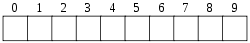
\includegraphics[width=0.48\textwidth]{pic1.png}
\end{center}
\caption{tablica 10-elementow}
\label{Etykieta}
\end{wrapfigure}

W rozdziale Zmienne w C dowiedziałeś się, jak przechowywać pojedyncze liczby oraz znaki. Czasami zdarza się jednak, że potrzebujemy przechować kilka, kilkanaście albo i więcej zmiennych jednego typu. Nie tworzymy wtedy np. dwudziestu osobnych zmiennych. W takich przypadkach z pomocą przychodzi nam tablica.



Tablica to ciąg zmiennych jednego typu. Ciąg taki posiada jedną nazwę a do jego poszczególnych elementów odnosimy się przez numer (indeks).

\section*{Wstęp}

\subsection*{Sposoby deklaracji tablic}\\

Tablicę deklaruje się w następujący sposób:
\begin{lstlisting}[caption=Deklaracja, captionpos=t, label=src:sqrt, frame=lBTr, frameround=ffff, captionpos=b]
typ nazwa_tablicy[rozmiar];
\end{lstlisting}
gdzie rozmiar oznacza ile zmiennych danego typu możemy zmieścić w tablicy. Zatem aby np. zadeklarować tablicę, mieszczącą 20 liczb całkowitych możemy napisać tak:
\begin{lstlisting}[caption=Deklaracja tablicy 20 int, captionpos=t, label=src:sqrt, frame=lBTr, frameround=ffff, captionpos=b]
int tablica[20];
\end{lstlisting}
Podobnie jak przy deklaracji zmiennych, także tablicy możemy nadać wartości początkowe przy jej deklaracji. Odbywa się to przez umieszczenie wartości kolejnych elementów oddzielonych przecinkami wewnątrz nawiasów klamrowych:
\begin{lstlisting}[caption=Inicjalizacja, captionpos=t, label=src:sqrt, frame=lBTr, frameround=ffff, captionpos=b ]
 int tablica[3] = {0,1,2};
\end{lstlisting}
Niekoniecznie trzeba podawać rozmiar tablicy, np.:
\begin{lstlisting}[caption=Inicjalizacja bez rozmiaru, captionpos=t, label=src:sqrt, frame=lBTr, frameround=ffff, captionpos=b ]
 int tablica[] = {1, 2, 3, 4, 5};
\end{lstlisting}
W takim przypadku kompilator sam ustali rozmiar tablicy (w tym przypadku - 5 elementów).

Rozpatrzmy następujący kod:
\begin{lstlisting}[caption=Printowanie tablicy, captionpos=t, label=src:sqrt, frame=lBTr, frameround=ffff, captionpos=b ]
 #include <stdio.h>
 #define ROZMIAR 3
 int main()
 {
   int tab[ROZMIAR] = {3,6,8};
   int i;
   puts ("Druk tablicy tab:");
 
   for (i=0; i<ROZMIAR; ++i) {
     printf ("Element numer %d = %d\n", i, tab[i]);
   }
   return 0;
 }
\end{lstlisting}

Wynik:
\begin{lstlisting}[caption=Wyniki, captionpos=t, label=src:sqrt, frame=lBTr, frameround=ffff, captionpos=b ]
Druk tablicy tab:
Element numer 0 = 3
Element numer 1 = 6
Element numer 2 = 8
\end{lstlisting}
Jak widać, wszystko się zgadza.

W powyżej zamieszczonym przykładzie użyliśmy stałej do podania rozmiaru tablicy. Jest to o tyle pożądany zwyczaj, że w razie potrzeby zmiany rozmiaru tablicy, zmieniana jest tylko wartość w jednej linijce kodu przy #define, w innym przypadku musielibyśmy szukać wszystkich wystąpień rozmiaru rozsianych po kodzie całego programu.

\subsection*{Odczyt/zapis wartości do tablicy}
Tablicami posługujemy się tak samo jak zwykłymi zmiennymi. Różnica polega jedynie na podawaniu indeksu tablicy. Określa on, z którego elementu (wartości) chcemy skorzystać spośród wszystkich umieszczonych w tablicy. Numeracja indeksów rozpoczyna się od zera, co oznacza, że pierwszy element tablicy ma indeks równy 0, drugi 1, trzeci 2, itd.

Spróbujmy przedstawić to na działającym przykładzie. Przeanalizuj następujący kod:

\begin{lstlisting}[caption=Fragment, captionpos=t, label=src:sqrt, frame=lBTr, frameround=ffff, captionpos=b ]
 int tablica[5] = {0};
 int i = 0;
 tablica[2] = 3;
 tablica[3] = 7;
 for (i=0;i!=5;++i) {
   printf ("tablica[%d]=%d\n", i, tablica[i]);
 }

\end{lstlisting}
Jak widać, na początku deklarujemy 5-elementową tablicę, którą od razu zerujemy. Następnie pod trzeci i czwarty element (liczone począwszy od 0) podstawiamy liczby 3 i 7. Pętla ma za zadanie wyprowadzić wynik naszych działań.

\subsection*{Tablice znaków}
Tablice znaków, tj. typu char oraz unsigned char, posiadają dwie ogólnie przyjęte nazwy, zależnie od ich przeznaczenia:
\begin{itemize}
\item{bufory - gdy wykorzystujemy je do przechowywania ogólnie pojętych danych, gdy traktujemy je jako po prostu "ciągi bajtów" (typ char ma rozmiar 1 bajta, więc jest elastyczny do przechowywania np. danych wczytanych z pliku przed ich przetworzeniem)}
\item{napisy - gdy zawarte w nich dane traktujemy jako ciągi liter; jest im poświęcony osobny rozdział Napisy.}
\end{itemize}
\newpage
Przykład:

\begin{lstlisting}[caption=Fragment kodu, captionpos=t, label=src:sqrt, frame=lBTr, frameround=ffff, captionpos=b ]
 /*
 http://joequery.me/code/snprintf-c/
 
 
  gcc a.c -Wall
 ./a.out
 
012345678
hello th\0
turtle\078
2222\05678

*/ 
#include<stdio.h>
#define BUFSIZE 9




void init_buf(char *buf, size_t size){
    int i;
    for(i=0; i<size; i++){
        buf[i] = i + '0'; // int to char conversion
    }
}

void print_buf(char *buf){
    int i;
    char c;
    for(i=0; i<BUFSIZE; i++){
        c = buf[i];
        if(c == '\0'){
            printf("\\0");

        }
        else{
            printf("%c", buf[i]);
        }
    }
    printf("\n");
}


int main(){
    char buf[BUFSIZE];
    init_buf(buf, BUFSIZE);
    print_buf(buf);

    // hello there! == 12 characters, > BUFSIZE
    init_buf(buf, BUFSIZE);
    snprintf(buf, BUFSIZE, "hello there!");
    print_buf(buf);

    // turtle == 6 charaters, < BUFSIZE
    init_buf(buf, BUFSIZE);
    snprintf(buf, BUFSIZE, "turtle");
    print_buf(buf);

    // 2222220 == 7 charaters, > 5
    init_buf(buf, BUFSIZE);
    snprintf(buf, 5, "%d", 222222 * 10);
    print_buf(buf);

    return 0;
}

\end{lstlisting}
\begin{wrapfigure}{r}{0.3\textwidth}
\begin{center}
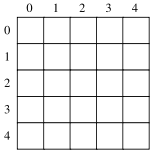
\includegraphics[width=0.3\textwidth]{pic2.png}
\end{center}
\caption{tablica 10-elementow}
\label{Etykieta}
\end{wrapfigure}
\subsection*{Tablice wielowymiarowe}

Rozważmy teraz konieczność przechowania w pamięci komputera całej macierzy o wymiarach 10 x 10. Można by tego dokonać tworząc 10 osobnych tablic jednowymiarowych, reprezentujących poszczególne wiersze macierzy. Jednak język C dostarcza nam dużo wygodniejszej metody, która w dodatku jest bardzo łatwa w użyciu. Są to tablice wielowymiarowe, lub inaczej "tablice tablic". Tablice wielowymiarowe definiujemy podając przy zmiennej kilka wymiarów, np.:


\begin{lstlisting}[caption=Macierz, captionpos=t, label=src:sqrt, frame=lBTr, frameround=ffff, captionpos=b ]
 float macierz[10][10];
\end{lstlisting}
Tak samo wygląda dostęp do poszczególnych elementów tablicy:
\begin{lstlisting}[caption=Macierz, captionpos=t, label=src:sqrt, frame=lBTr, frameround=ffff, captionpos=b ]
macierz[2][3] = 1.2;
\end{lstlisting}
Jak widać ten sposób jest dużo wygodniejszy (i zapewne dużo bardziej "naturalny") niż deklarowanie 10 osobnych tablic jednowymiarowych. Aby zainicjować tablicę wielowymiarową należy zastosować zagłębianie klamr, np.:
\begin{lstlisting}[caption=Macierz, captionpos=t, label=src:sqrt, frame=lBTr, frameround=ffff, captionpos=b ]
 float macierz[3][4] = {
   { 1.6, 4.5, 2.4, 5.6 },  /* pierwszy wiersz */
   { 5.7, 4.3, 3.6, 4.3 },  /* drugi wiersz */
   { 8.8, 7.5, 4.3, 8.6 }   /* trzeci wiersz */
 };
\end{lstlisting}
Dodatkowo, pierwszego wymiaru nie musimy określać (podobnie jak dla tablic jednowymiarowych) i wówczas kompilator sam ustali odpowiednią wielkość, np.:

\begin{lstlisting}[caption=Macierz, captionpos=t, label=src:sqrt, frame=lBTr, frameround=ffff, captionpos=b ]
 float macierz[][4] = {
   { 1.6, 4.5, 2.4, 5.6 },  /* pierwszy wiersz */
   { 5.7, 4.3, 3.6, 4.3 },  /* drugi wiersz */
   { 8.8, 7.5, 4.3, 8.6 },  /* trzeci wiersz */
   { 6.3, 2.7, 5.7, 2.7 }  /* czwarty wiersz */
 };
\end{lstlisting}
Innym, bardziej elastycznym sposobem deklarowania tablic wielowymiarowych, jest użycie wskaźników. Opisane to zostało w następnym rozdziale.

\subsection*{Kolejność głównych wierszy}
Kolejność głównych wierszy ( ang. Row Major Order = ROM [1])

W C tablica wielowymiarowa A[n][m] :
\begin{itemize}
\item{jest przechowywana wierszami}
\item{numeracja indeksów rozpoczyna się od zer}
\end{itemize}
   
   \begin{lstlisting}[caption=Tablica, captionpos=t, label=src:sqrt, frame=lBTr, frameround=ffff, captionpos=b ]
 A[0][0], A[0][1], ..., A[0][m-1], A[1][0], A[1][1],..., A[n-1][m-1] 
\end{lstlisting}

Przykładowy program :

\begin{lstlisting}[caption=Kod, captionpos=t, label=src:sqrt, frame=lBTr, frameround=ffff, captionpos=b ]
/*
 http://stackoverflow.com/questions/2151084/map-a-2d-
 array-onto-a-1d-array-c/2151113

*/
  #include <stdio.h>

   int main(int argc, char **argv) {
   int i, j, k;
   int arr[5][3];
   int *arr2 = (int*)arr;

       for (k=0; k<15; k++) {
          arr2[k] = k;
          printf("arr[%d] = %2d\n", k, arr2[k]);
       }

       for (i=0; i<5; i++) {
         for (j=0; j< 3; j++) {
            printf("arr2[%d][%d] = %2d\n", i, j ,arr[i][j]);
         }
       } 
    }
\end{lstlisting}


\subsection*{Ograniczenia tablic}
Pomimo swej wygody tablice statyczne mają ograniczony, z góry zdefiniowany rozmiar, którego nie można zmienić w trakcie działania programu. Dlatego też w niektórych zastosowaniach tablice statyczne zostały wyparte tablicami dynamicznymi, których rozmiar może być określony w trakcie działania programu. Zagadnienie to zostało opisane w następnym rozdziale.

Wystarczy pomylić się o jedno miejsce (tzw. błąd off by one) by spowodować, że działanie programu zostanie nagle przerwane przez system operacyjny ( błąd przy uruchamianiu ) :


\begin{lstlisting}[caption=Bład, captionpos=t, label=src:sqrt, frame=lBTr, frameround=ffff, captionpos=b ]
 int foo[100];
 int i;
 
 for (i=0; i<=100; i+=1) /* powinno być i<100 */
   foo[i] = 0;

 /* program powinien zakończyć się błędem */
\end{lstlisting}


\end{document}